\documentclass{beamer}
\usepackage{beamerthemesplit}
\usepackage{graphics}
%\usepackage[lined,boxed]{algorithm2e}
\usepackage[lined]{algorithm2e}
\usepackage{amsmath}
\usepackage{amssymb}
\usepackage{listings}
\usepackage{soul}
\lstset{
basicstyle=\small,
keywordstyle=\color{blue}\bfseries,
numbers=left,
numberstyle=\tiny,
numbersep=5pt,
showstringspaces=false,
showspaces=false,
captionpos=b,
frame=tb,
float=tbh,
,escapeinside={*@}{@*}
}
\usetheme{Boadilla}
\title{Algorithms}
\subtitle{Review of Time Complexity and Formal Notations}
\author{Hikmat Farhat}
%\email{hfarhat@ndu.edu.lb}
%\institution{Notre Dame University}
\newtheorem{mydef}{Definition}
\newtheorem{lem}{Lemma}
%\newcommand{\emphasis}[1]{\textcolor{yellow}{#1}}
%\newcommand{\emphasis}[1]{\hl{#1}}
\newcommand{\emphasis}[1]{\ul{#1}}
\newcommand{\floor}[1]{\lfloor{#1}\rfloor}
\newcommand{\bfloor}[1]{\Big\lfloor{#1}\Big\rfloor}

%\newcommand{\gets}[0]{\leftarrow}

%\newcommand{\gets}{\ensuremath{\leftarrow}}
%\DeclareTextFontCommand{\emph}{\emphasis}
\sethlcolor{yellow}
\begin{document}

\section{Efficient Algorithms}
% title page
\frame{\titlepage}

% slide 

\begin{frame}
  \frametitle{Efficient Algorithms}

  \begin{itemize}
\item Given an algorithm to solve a problem we ask
\item Is it efficient?
\item We seek a sensible definition of efficiency
\item How much work if the input doubles in size?
\item For large input sizes can our algorithm solve the problem in a
  reasonable time?
  \end{itemize}
\end{frame}

% slide

\begin{frame}
\frametitle{Polynomial Time}
\begin{itemize}
\item Efficient algorithm =\emphasis{ polynomial} in the size of the input
     \begin{mydef}
       \textbf{Polynomial Time}: for every input of size $n$\\
 $\exists a,b$ such
   that number of computation steps $<an^b$
     \end{mydef}
\item $a$ and $b$ are constants that do not depend on $n$
  \item True, some algorithms are polynomials with $a$ and/or $b$ very large
\item but for the \emphasis{majority} of algorithms, $a$ and $d$ are
  relatively small
% \item exponential is expensive
% \item ignore constant and power because we ignore detail

% \item Does not take "too much" time.
\end{itemize}
\end{frame}
\begin{frame}
\frametitle{Why Polynomial Time ?}
  \begin{center}
  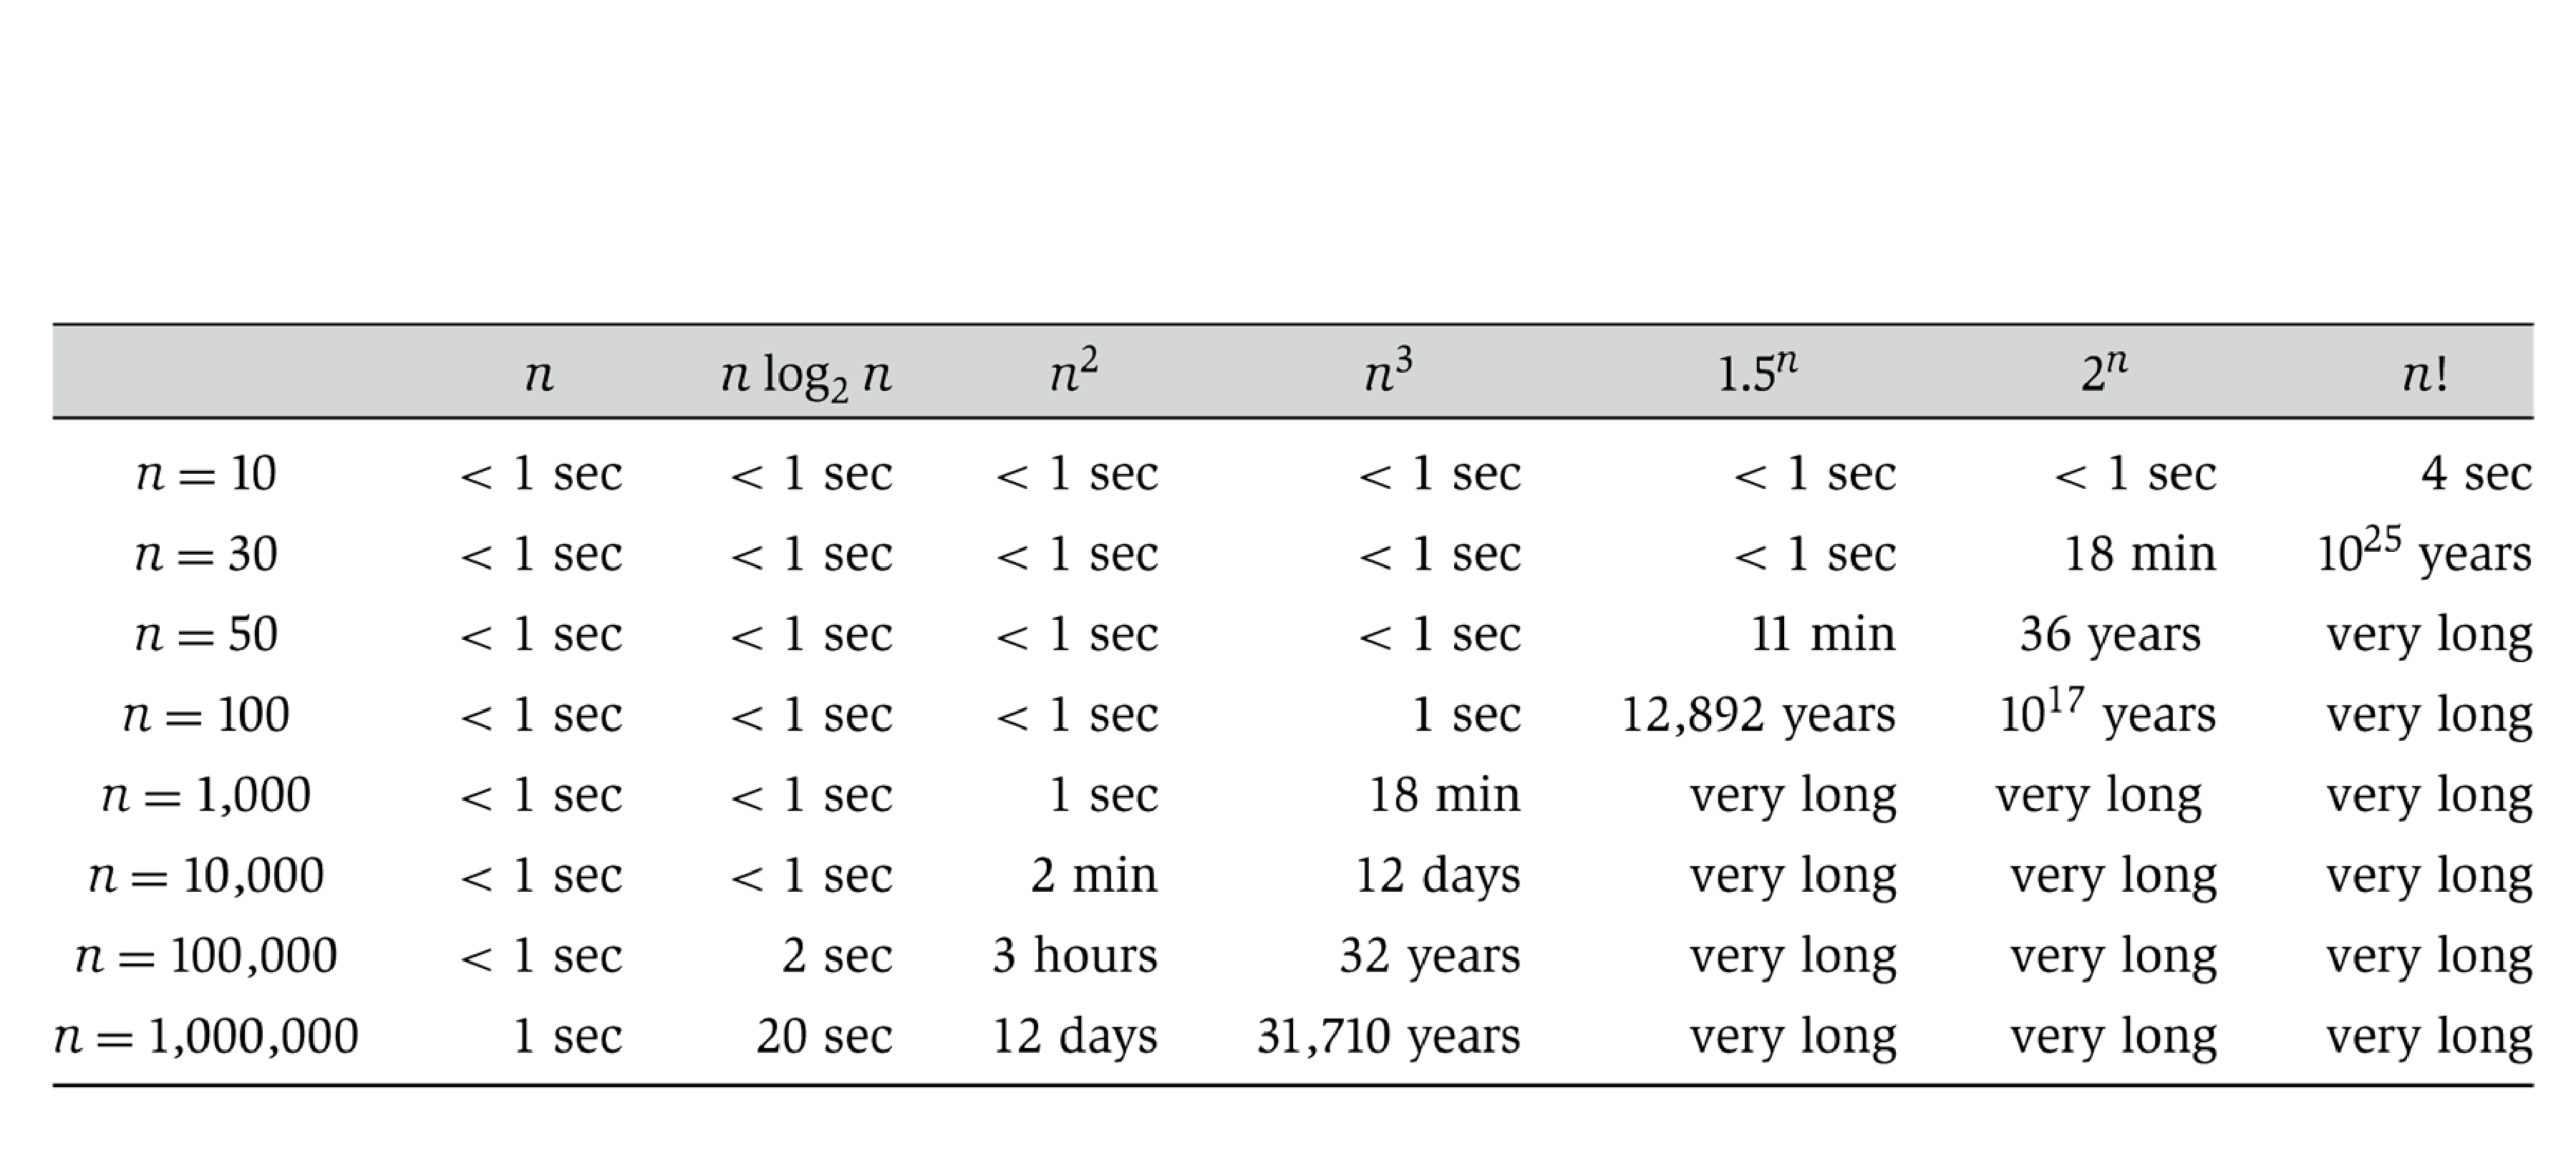
\includegraphics[width=\textwidth]{complexity-figs/growth-table.pdf}    
  \end{center}

\end{frame}

\begin{frame}
\frametitle{Worst Case Analysis}
\begin{itemize}
\item Usually the running time is the running time of the
  \emphasis{worst case}
\item One could analysis the \emphasis{average case} but it much more
  difficult and depends on the chosen distribution.
\item Therefore an algorithm is efficient if it has a \emphasis{worst case
  polynomial time}
\item There are exceptions the most important being the simplex
  algorithm that works very well in practice
\end{itemize}
\end{frame}

\section{Asymptotic Growth}
\begin{frame}

\frametitle{Asymptotic Growth of Functions}
\begin{mydef}
\emphasis{Big Oh:}The set $O(g(n))$ is defined as all functions $f(n)$ with the property\\
$\exists c,n_0$ such that $f(n)\le c g(n)$ for all $n\ge n_0$
\end{mydef}
\begin{figure}[h]
  \centering
  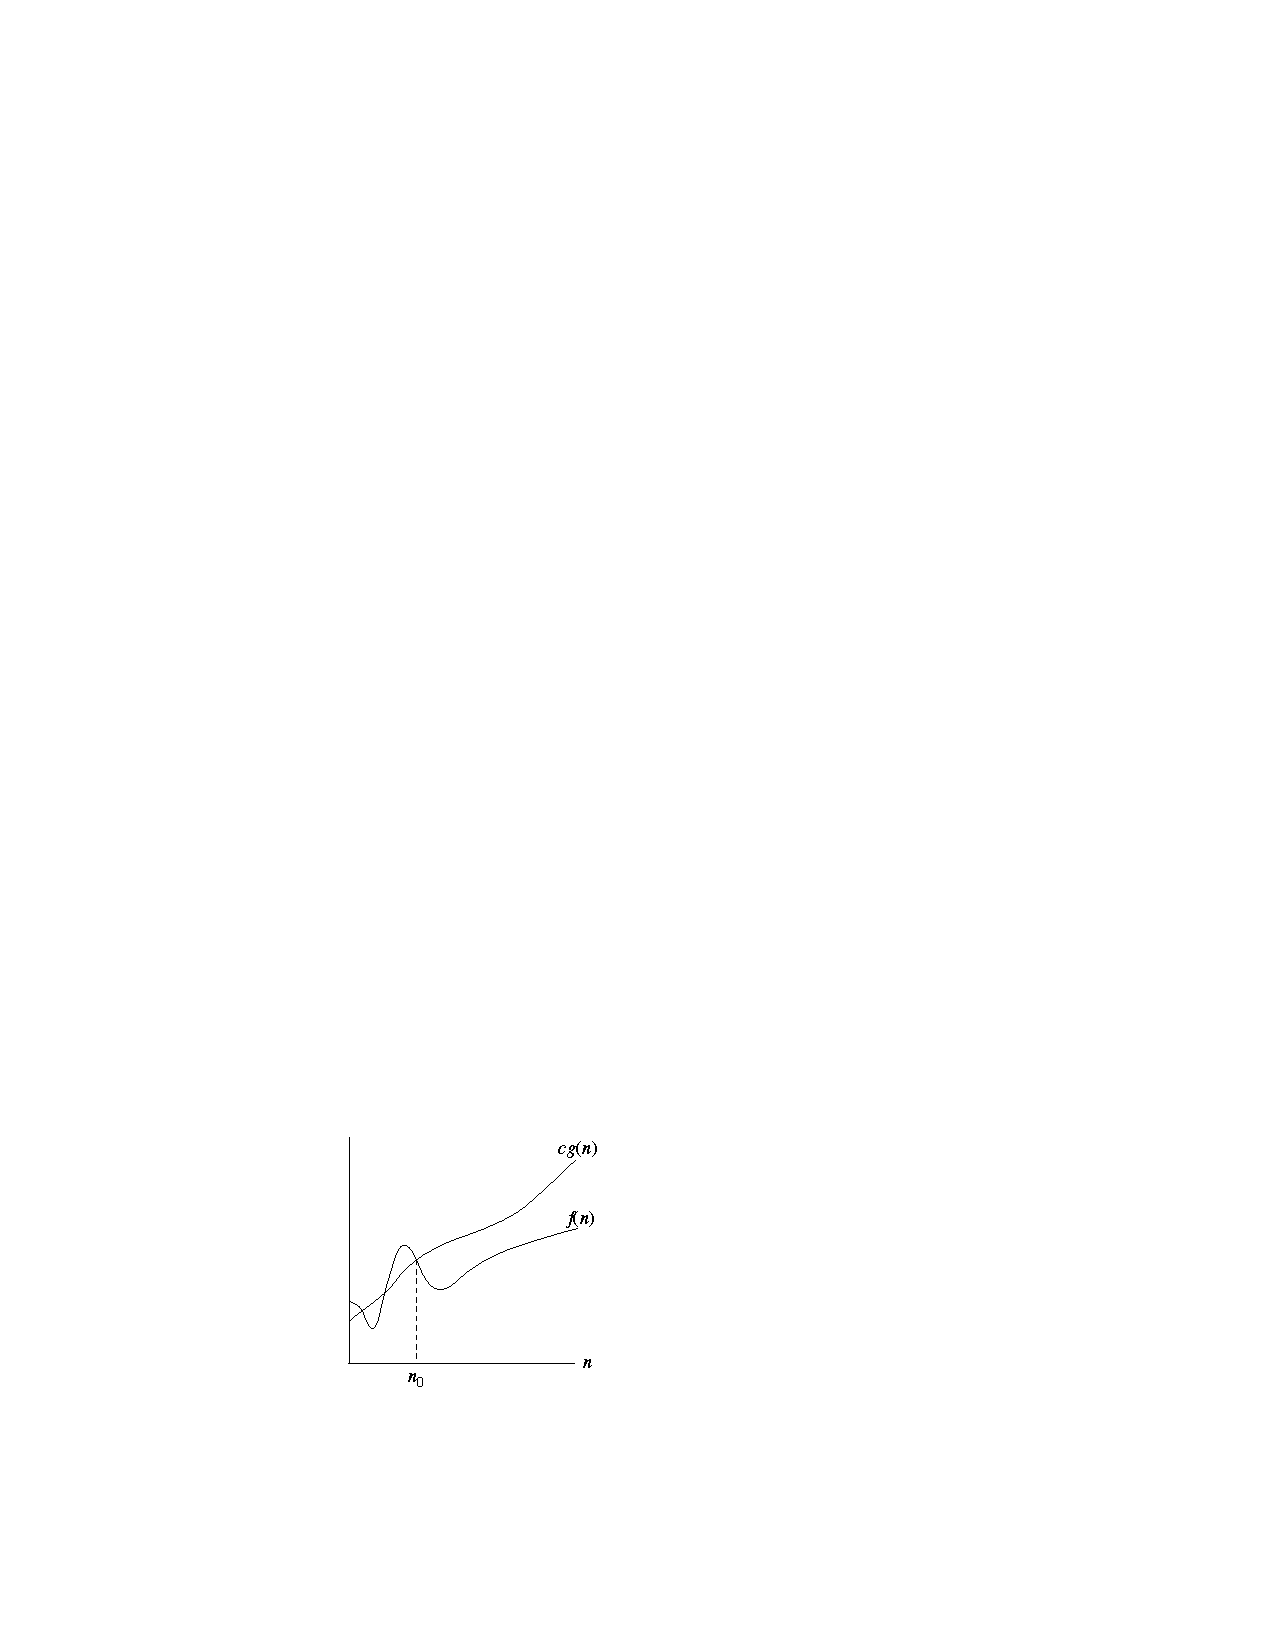
\includegraphics[width=0.5\textwidth]{complexity-figs/Big-Oh.pdf}
\caption{Graphical definition of $O$ taken from the CLRS book}
\end{figure}
\end{frame}


\begin{frame}
  \frametitle{Example}
  \begin{itemize}
  \item $f(n)=2n^2+n=O(n^2)$ because let $c=3$ and $n_0=1$
    \begin{align*}
     \forall n\ge n_0=1\\
     n&\le n^2\\
     2n^2+n&\le 3n^2\\
     f(n)&\le c n^2\\
     f(n)&=O(n^2)
    \end{align*}
  \item On the other hand $f(n)=2n^2+n\ne O(n)$
  \end{itemize}
\end{frame}


\begin{frame}
  
\begin{mydef}
\emphasis{Big Omega:}The set $\Omega(g(n))$ is defined as all functions $f(n)$ with the property\\
$\exists c,n_0$ such that $ f(n)\ge c g(n)$ for all $n\ge n_0$
\end{mydef}
\begin{figure}[h]
  \centering
  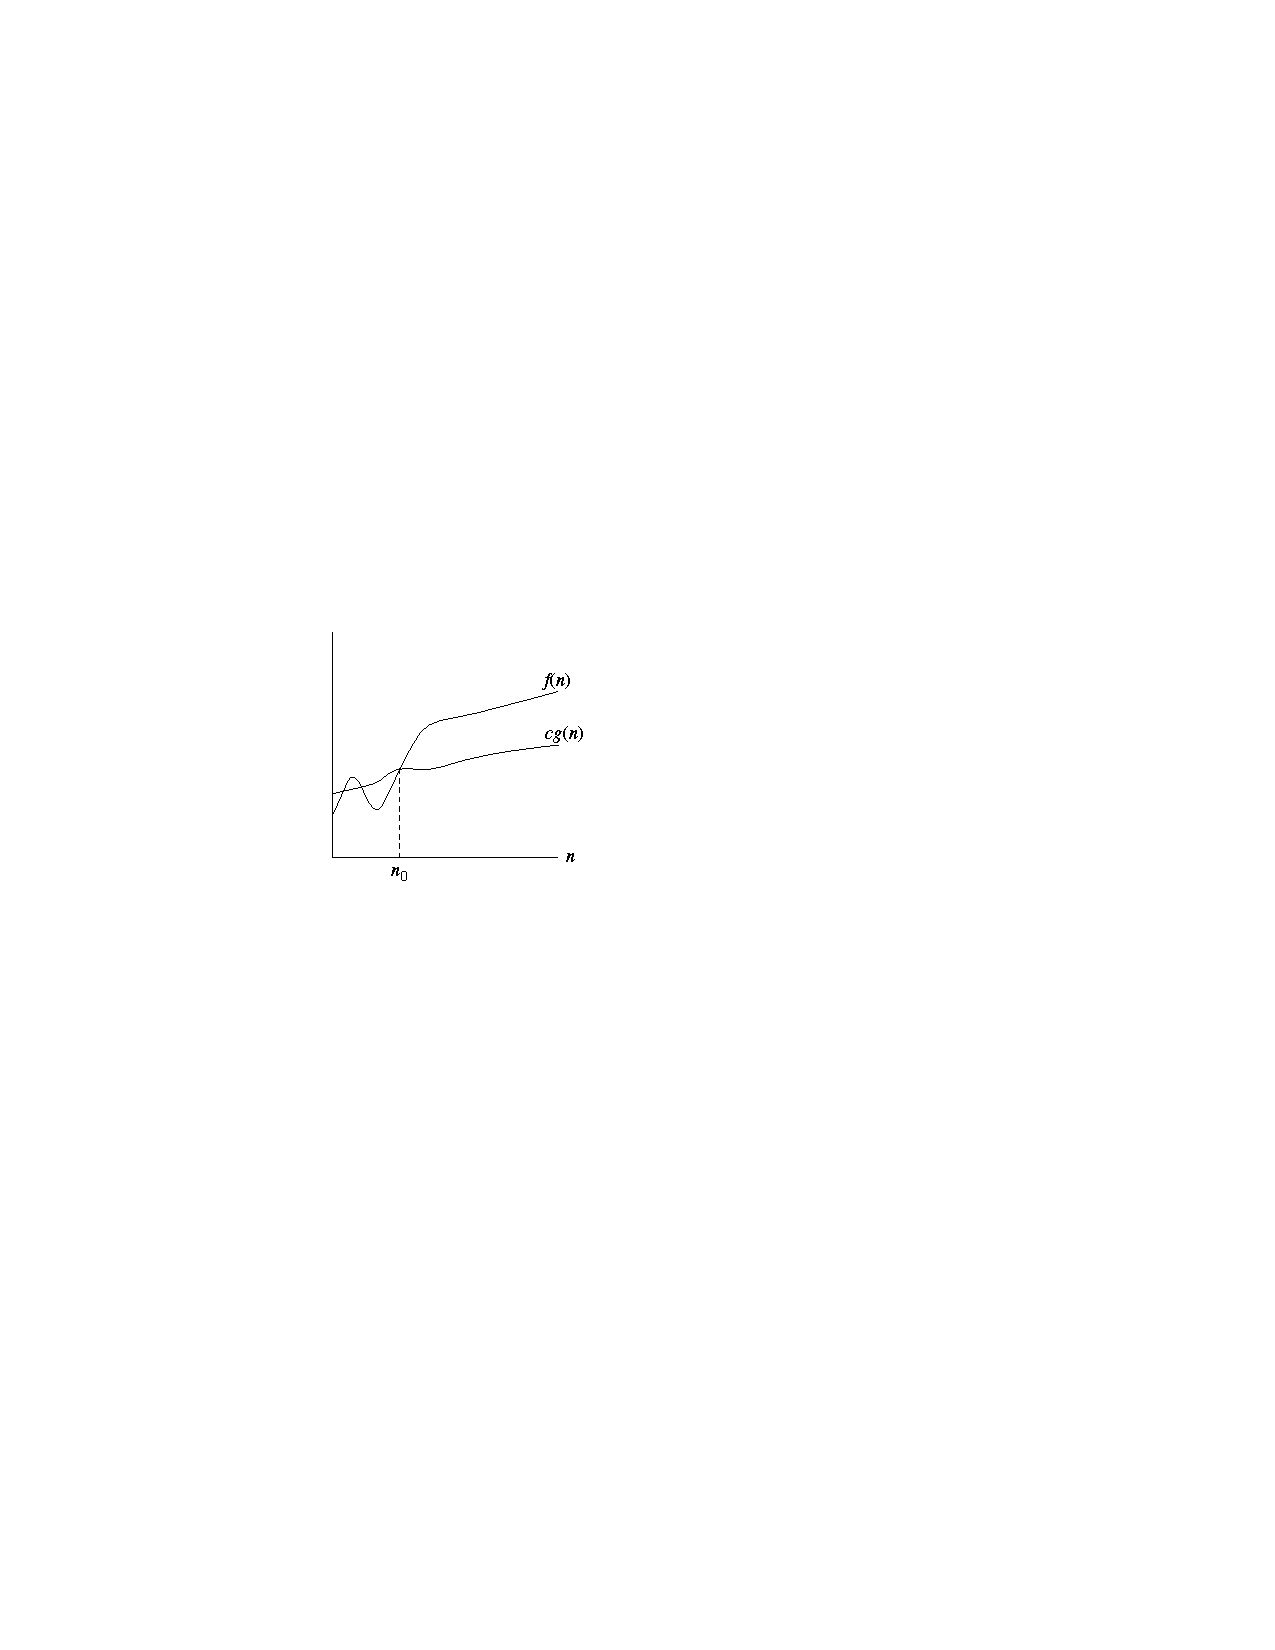
\includegraphics[width=0.5\textwidth]{complexity-figs/Big-Omega.pdf}
\caption{Graphical definition of $\Omega$ taken from the CLRS book}
\end{figure}
\end{frame}

\begin{frame}
  \frametitle{Example}
  \begin{itemize}
  \item Consider $f(n)=\sqrt{n}$ and $g(n)=\log n$.
\item $f(n)=\Omega(g(n))$ because for $c=1,n_0=16$ we have

  \begin{align*}
    \sqrt{16}=4=\log 2^4
  \end{align*}

\item Note that between n=4 and n=16 the value of $\log_2 n\ge \sqrt{n}$
  \end{itemize}
\end{frame}
% \begin{frame}
%   \begin{center}
%   \includegraphics[width=0.9\textwidth]{complexity-figs/log-vs-sqrt.png}    
%   \end{center}

% \end{frame}


\frame{

  \begin{itemize}
  \item Abuse of notation: if $h(n)\in O(g(n))$ we write
    $h(n)=O(g(n))$
  \item similarly if $h(n)\in \Omega(g(n))$ we write\\
 $h(n)=\Omega(g(n))$

\item If $h(n)=O(g(n))$ we say $g(n)$ is an \emphasis{upper bound} for $f(n)$.
\item If $h(n)=\Omega(g(n))$ we say $g(n)$ is a \emphasis{lower bound} for
  $f(n)$.
  \end{itemize}
}

\frame{
\begin{mydef}
\emphasis{Big $\Theta$:}The set $\Theta(g(n))$ is defined as all functions $f(n)$ with the property\\
$\exists c_1,c_2,n_0$ such that $c_1 g(n)\le f(n)\le c_2 g(n)$ for all $n\ge n_0$
\end{mydef}
\begin{figure}[h]
  \centering
  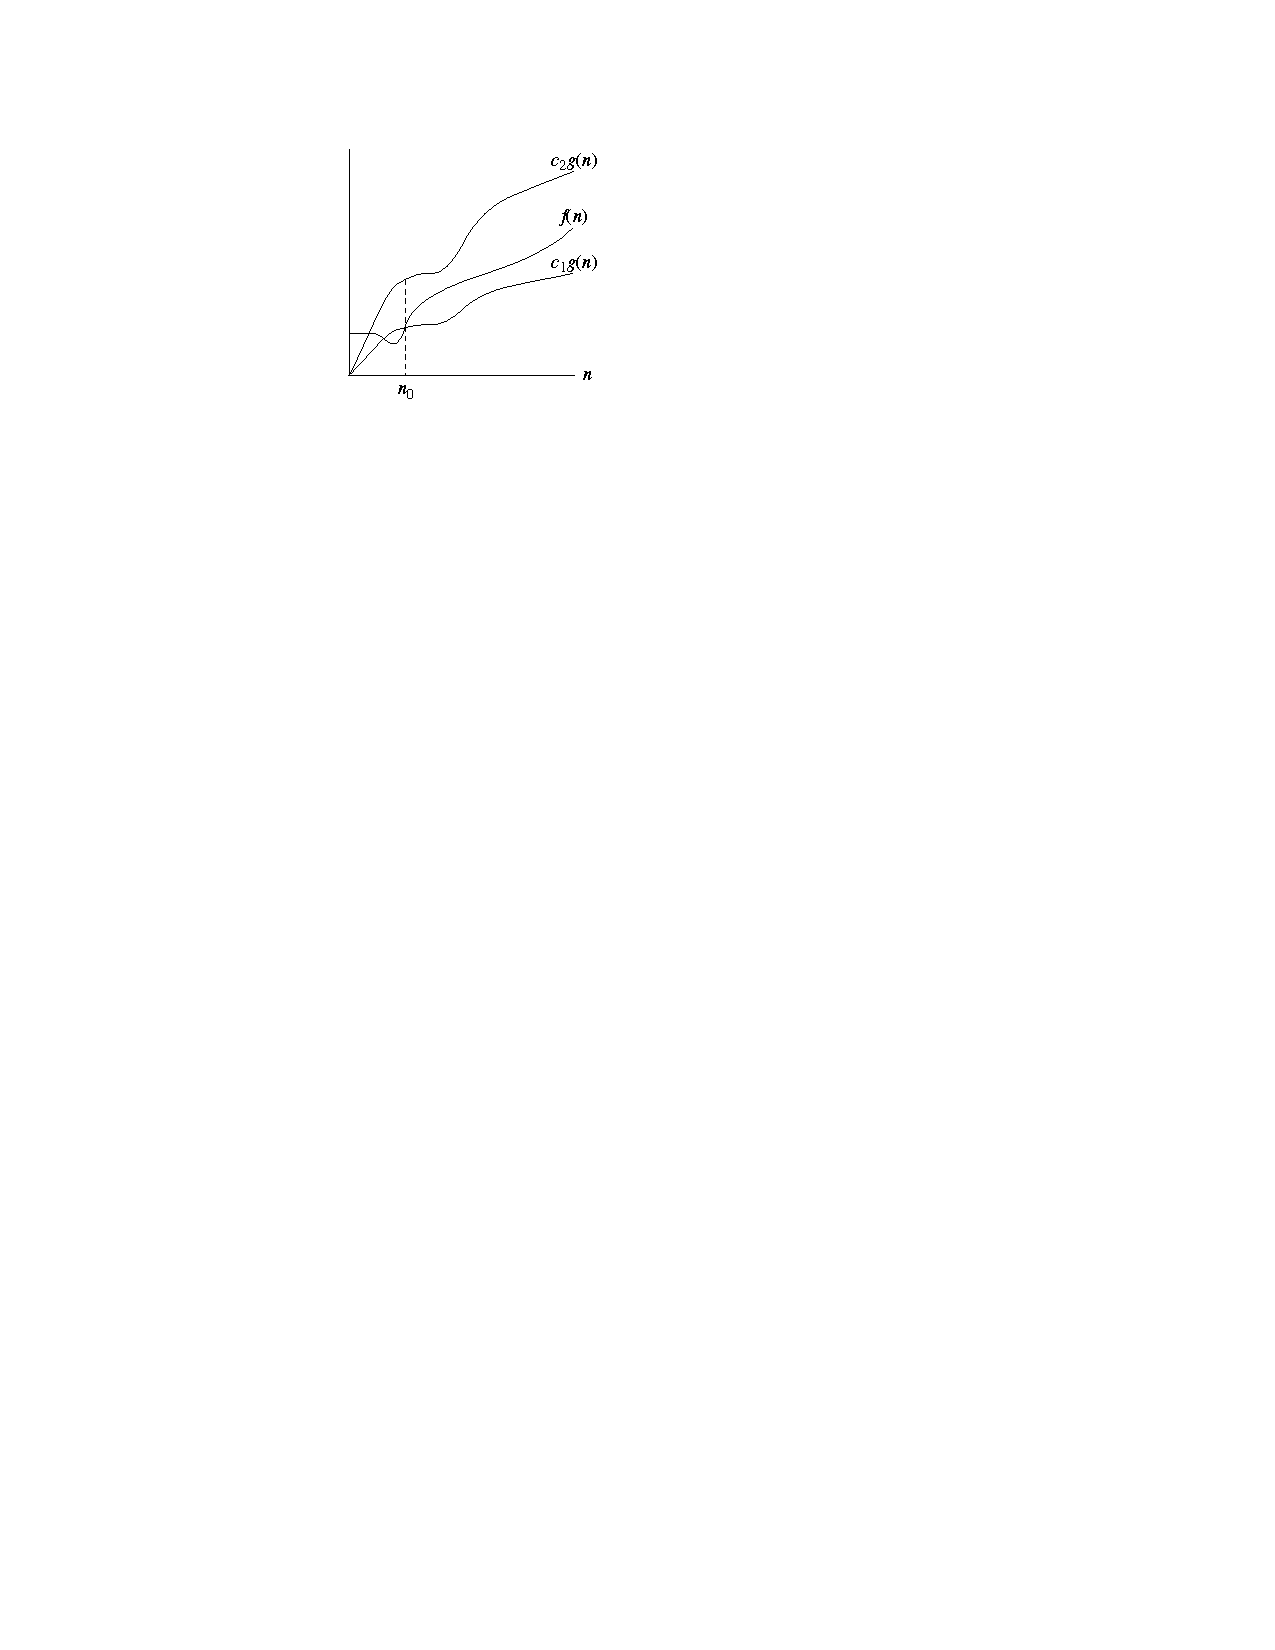
\includegraphics[width=0.5\textwidth]{complexity-figs/Big-Theta.pdf}
\caption{Graphical definition of $\Theta$ taken from the CLRS book}
\end{figure}

}
\begin{frame}
  \frametitle{Example}
  \begin{itemize}
  \item Consider $c_1=1$, $c_2=3$ and $n_0=1$ it is obvious that 
    \begin{align*}
      c_1n^2\le 2n^2+n\le c_2n^2\ \forall n\ge n_0
    \end{align*}
  \item We can show that $f(n)=\Theta(g(n))$ iff\\
    $f(n)= O(g(n))$ and \\
    $f(n)=\Omega(g(n))$
  \item If $f(n)=\Theta(g(n))$ we say $g(n)$ is a \emphasis{tight bound}
    for $f(n)$.
\end{itemize}
\end{frame}
\frame{
  \begin{mydef}
   \emphasis{Little Oh:} The set $o(g(n))$ is defined as all functions
   $f(n)$ with the property\\
\emphasis{for all} $c$, $\exists n_0 $ such that \\
$f(n)< cg(n)$ for all $n\ge n_0$
  \end{mydef}
We can show that the above definition is equivalent to 
\begin{displaymath}
\lim_{n\rightarrow\infty}\frac{f(n)}{g(n)}=0  
\end{displaymath}

}


\begin{frame}
  \begin{mydef}
   \emphasis{Little omega:} The set $\omega(g(n))$ is defined as all functions
   $f(n)$ with the property\\
\emphasis{for all} $c$, $\exists n_0 $ such that \\
$cg(n)<f(n)$ for all $n\ge n_0$
  \end{mydef}
We can show that the above definition is equivalent to 
\begin{displaymath}
\lim_{n\rightarrow\infty}\frac{f(n)}{g(n)}=\infty
\end{displaymath}

\end{frame}


\frame{
\frametitle{Examples}
\begin{itemize}
\item $f(n)=2n^2+n$
\item $f(n)=\omega(n)$ because 
  \begin{align*}
\lim_{n\rightarrow\infty}\frac{2n^2+n}{n}=\infty
  \end{align*}


\item $f(n)=o(n^3)$ because
  \begin{align*}
\lim_{n\rightarrow\infty}\frac{2n^2+n}{n^3}=0
  \end{align*}


\end{itemize}
}

\frame{
\frametitle{Using Limits}
\begin{itemize}
\item Sometimes it is easier to determine the relative growth rate of two functions $f(n)$ and $g(n)$
by using limits
\begin{itemize}
\item if $\lim_{n\rightarrow\infty}\frac{f(n)}{g(n)}=0$ then $f(n)=o(g(n))$.
\item if $\lim_{n\rightarrow\infty}\frac{f(n)}{g(n)}=\infty$ then $f(n)=\omega(g(n))$.
\item if $\lim_{n\rightarrow\infty}\frac{f(n)}{g(n)}=c$, for some constant $c$, then $f(n)=\Theta(g(n))$.
\end{itemize}
\item Can we always do that?No
\item In many situations the complexity cannot be written in an
  analytic form.
\end{itemize}

}
\frame{
\frametitle{Exponential vs Polynomial vs Logarithmic}
it is easy  to show that for all $a>0$ ,$b>1$ 
%(hint: use l'Hopital rule and consider $n^{\lceil a\rceil}>n^a$)
\begin{displaymath}
  \lim_{n\rightarrow\infty}\frac{n^a}{b^n}=0
\end{displaymath}
And polynomials grow faster(use $m=\log n$ and the previous result)
than logarithms ($\log^a x=(\log x)^a$)
\begin{align*}
  \lim_{n\rightarrow\infty}\frac{\log^an}{n^b}&=0\\
%                                          &=\lim_{m\rightarrow\infty}\frac{m^a}{2^{m^b}}\\
%                                         &=\lim_{m\rightarrow\infty}\frac{m^a}{(2^b)^m}\\
%                                         &=\lim_{m\rightarrow\infty}\frac{m^a}{c^m}\\
%                                         &=0
\end{align*}
}
%slide

\frame{
\frametitle{Arithmetic Properties}
\begin{itemize}
\item \emphasis{transitivity}: if $f(n)=O(g(n))$ and $g(n)=O(h(n))$
  then $f(n)=O(h(n))$.
  \begin{itemize}
  \item eg: $\log n=O(n)$ and $n=O(2^n)$ then $\log n=O(2^n)$.
  \end{itemize}
\item \emphasis{constant factor}: if $f(n)=O(kg(n))$ for some $k>0$
  then $f(n)=O(g(n))$.
  \begin{itemize}
  \item eg: $n^2=O(3n^2)$ thus $n^2=O(n^2)$.
  \end{itemize}
\item \emphasis{sum}: if $f_1(n)=O(g_1(n))$ and $f_2(n)=O(g_2(n))$ then
$f_1(n)+f_2(n)=O(\max(g_1(n),g_2(n)))$
\begin{itemize}
\item $3n^2=O(n^2)$, $6\log n=O(\log n)$ then $3n^2+6\log n=O(n^2)$
\end{itemize}
\item \emphasis{product}:$f_1(n)=O(g_1(n))$ and $f_2(n)=O(g_2(n))$
  then $f_1(n)*f_2(n)=O(g_1(n)*g_2(n))$
  \begin{itemize}
  \item eg:  $3n^2=O(n^2)$, $6\log n=O(\log n)$ then $3n^2*6\log
    n=O(n^2\log n)$
  \end{itemize}
\end{itemize}

}
\subsection{Code Fragments}
\begin{frame}[fragile]
\frametitle{Code Fragments}
\begin{function}[H]

\DontPrintSemicolon
  \SetKwFunction{Max}{max}
  \BlankLine
  $sum=0$\;
  \For{$i=1\ldots n$}{
      $sum\gets sum+1$\;
   }
\end{function}
\begin{itemize}
\item the operation $sum=0$ is independent of the input thus it costs
  a constant time $c_1$.
\item the operation $sum\gets sum+1$ is independent of the input thus it cost some constant time $c_2$.
\item Regardless of the input the loop runs  $n$ times therefore the
  total cost is $c_1+c_2n=\Theta(n)$.
\end{itemize}
\end{frame}
\section{Example Algorithms}
\subsection{Maximum of N numbers}
\frame{
The algorithm below for finding the maximum of $n$ numbers is $\Theta(n)$.\\
Input: $a_1,\ldots,a_n$\\
Output: $max(a_1,\ldots,a_n)$
\begin{function}[H]
 
  \DontPrintSemicolon
  \SetKwFunction{Max}{max}
  \BlankLine
Initially $max=a_1$\;
  \For{$i=2\ldots n$}{
    \If{$a_i>max$}{
      $max=a_i$
    }
   }
\end{function}
   \begin{itemize}
   \item Try 89,47,80,50,67,102 and 19,15,13,10,8,3
   \item Do they have the "same" running time?
   \end{itemize}

}
\subsection{Sequential Search}
\frame{
\frametitle{Sequential Search}

Given an array $a$ check if element $x$ is in the array.
\begin{function}[H]
 \DontPrintSemicolon
  \SetKwFunction{Max}{max}
  \BlankLine
  \For{$i=1\ldots n$}{
    \If{$a[i]=x$}{
      \Return True
    }
   }
\Return False
\end{function}
\begin{itemize}
\item What is the running time of the above algorithm?
\item Consider the two extreme cases: $x$ is the first or the last
  element of the array.
\end{itemize}

}
\frame{
  \begin{itemize}
  \item If $x$ is the \emphasis{first} element than we perform \emphasis{a
      single} operation. This is the \emphasis{best-case}.
  \item If $x$ is the \emphasis{last} element than we perform
    \emphasis{$n$} operation.This is the \emphasis{worst-case}.
\item Now if we run the algorithm on many different (random) input and
  average out the results we get the \emphasis{average-case}.
\item Which one do we use?
  \begin{itemize}
  \item  Depends on the application and the feasibility.
   \item Real-time and critical applications usually require
     worst-case
   \item In most other situations we prefer average-case, but
     difficult to calculate and depends on the random distribution!
  \end{itemize}

\item In light of the above, what is the best-case,average-case and
  worst-case for the compute max algorithm we had before?
  \end{itemize}


}

\begin{frame}
  \frametitle{Nested Loops}
  \begin{itemize}
  \item What is the complexity of nested loops?
  \item The cost of a stmt in a nested loop is the cost of the
    statement multiplied by the product of the size of the loops
 
\begin{function}[H]
 
  \DontPrintSemicolon
 
  \For{$i=1\ldots n$}{
    \For{$j=1\ldots m$}{
      $k\gets k+1$
    }
   }
\end{function}
\item The cost is $\Theta(n*m)$
 \end{itemize}
\end{frame}


\subsection{Reflexive Transitive Closure}
\frame{
\frametitle{Reflexive Transitive Closure}

Given a set $A$, $|A|=n$, and a relation $R\subseteq A\times A$ we want to
compute the reflexive transitive closure,$R^*$, of $R$. Thus 
we want to compute all paths of size $1,\ldots,n$ and add them to $R^*$
\begin{function}[H]
 
  \DontPrintSemicolon
  \SetKwFunction{Update}{update}
  \BlankLine
Initially $ R^*=\emptyset$\;
  \For{$i=1\ldots n$}{
    \ForEach{$(b_1,\ldots, b_i)\in A^i$}{
      if $(b_1,\ldots,b_i)$ is a path then add $(b_1,b_i)$ to $R$
    }
   }
\end{function}
What is the worst-case running time?

}
\frame{
  \begin{itemize}
  \item For each loop we need to consider $n^i$ tuples 
  \item and for each tuple we need to check if it is a path:
    \begin{itemize}
    \item $(b_1,\ldots,b_i)$ is a path in $R$ if $(b_k,b_{k+1})\in R$ for all $1\le k< i$
    \item this involves at most $i$ tests
    \end{itemize}
  
\item Computing a path of length $i$ is $\Theta(i)$ therefore the computation is $\sum_{i=1}^nin^i=\Theta(n^n)$
\item can we do better?Yes!
\item Use the transitivity property: if $(b_i,b_j)\in R^*$ and $(b_j,b_k)\in R^*$ then 
add $(b_i,b_k)$ to $R^*$
  \end{itemize}
}

\frame{
\begin{function}[H]
  \DontPrintSemicolon
  \SetKwFunction{Update}{update}
  \BlankLine
Initially $ R^*=R\cup\{(a_i,a_i):a_i\in A\}$\;
$changed$=True\;
  \While{changed}{
    $changed \gets$ False \;
    \ForAll {$a_i,a_j,a_k$}{
      \If {$(a_i,a_j)\in R^*\wedge (a_j,a_k)\in R^*\wedge
        (a_i,a_k)\notin R ^*$}{
        $R^*\gets R^*\cup \{ (a_i,a_k)\}$\;
        $changed\gets True$\;
      }
    }
   }
\end{function}
\begin{itemize}
\item The for loop considers $n^3$ elements and the while loop runs at
  most $n^2$ since we have $n^2$ pairs. The result is $\Theta(n^5)$.

\end{itemize}
}

\subsection{Factorial}

\begin{frame}
  \frametitle{Factorial}
\begin{itemize}
\item Consider the recursive implementation of the factorial function.

  
\begin{function}[H]
  \DontPrintSemicolon
  \SetKwFunction{Factorial}{factorial}
  \Factorial{n}
  \BlankLine
 \eIf{n=1}{
    \Return{1}
    }
{
      \Return{n*\Factorial{n-1}}
    }
  \end{function}

\item The cost of size $n$? $T(n)=T(n-1)+C$
\item Thus $T(n)=\Theta(n)$.
\end{itemize}

\end{frame}

\begin{frame}
  \frametitle{Complexity of Factorial}
  \begin{align*}
    T(n)&=T(n-1)+C\\
        &=T(n-2)+2C\\
        &=\ldots \\
        &=T(n-i)+i*C\\
        &=\ldots \\
        &=T(1)+(n-1)*C\\
        &=n*C+T(1)-C\\
        &=\Theta(n)
  \end{align*}
\end{frame}
\begin{frame}
  \frametitle{Fibonacci}
  \begin{itemize}
  \item Computing the $n^{th}$ Fibonacci number can be done
    recursively 
 
\begin{function}[H]
 \DontPrintSemicolon
  \SetKwFunction{Fib}{fib}
  \Fib{n}
  \BlankLine
  \If{$n=0$}{
    \Return{0}
  }
 \If{$n=1$}{
    \Return{1}
    }

      \Return{\Fib{n-1}+\Fib{n-2}}

  \end{function}
\item If $T(n)$ is the cost of computing $Fib(n)$ then
  \begin{align*}
    T(n)=T(n-1)+T(n-2)+3
  \end{align*}
\item We will show, by \textbf{induction} on $n$, that $T(n)\ge fib(n)$
  i.e. the \textbf{cost} of computing Fibonacci number $n$ is greater
  than the \textbf{number} itself.
 \end{itemize}
\end{frame}
\begin{frame}
  \begin{itemize}
  \item We are assuming that all operations cost the same so the 3
    comes from executing the two if stmts and the sum.
\item First the base cases. If $n=0$ then the algorithm costs 1 (if
  stmt), if $n=1$ it costs 2 (2 if stmts) thus
    $T(0)=1$, $T(1)=2$.
\item In the other cases we have $T(n)=T(n-1)+T(n-2)+3$. This means
  $T(2)=6 \ge fib(2)=1$.
\item Assume that $T(n)\ge fib(n)$ then
  \begin{align*}
    T(n+1)&=T(n)+T(n-1)+3 & \\
          &\ge fib(n)+fib(n-1) & \text{ hyp. }\\
          &\ge fib(n+1)
  \end{align*}
%%% just by induction over n 
%%% f(n)=f(n-1)+f(n-2)
%%% f(n)> (3/2)^(n-1)+(3/2)^(n-2)
%% f(n)> [(2/3)+(4/9)](3/2)^n
%%% f(n)> (10/9)(3/2)^n
\item One can show that (for $n\ge 5$) $fib(n)\ge (3/2)^n$ thus $T(n)\ge (3/2)^n$
  which is exponential!
  \end{itemize}
\end{frame}

\begin{frame}
  \frametitle{Fibonacci: take two}
  \begin{itemize}
  \item can we compute Fibonacci numbers more efficiently?
  \item It turns out yes. By just "remembering" the values we already
    computed.
   \item A simple iterative algorithm
  \end{itemize}
\begin{function}[H]
  \DontPrintSemicolon
  \SetKwFunction{FiboIter}{FiboIter}
  \BlankLine
\FiboIter{n}\;
$f[0]\gets 0$\;
$f[1]\gets 1$\;
\For{$i\gets 2$ \KwTo $n$}{
  $f[i]\gets f[i-1]+f[i-2]$\;
}

\end{function}
  
\end{frame}
\begin{frame}
  \frametitle{Comparison}
  \begin{itemize}
  \item We had two different algorithms to compute Fibonacci number
    $n$
  \item One was $\Omega((3/2)^n)$ while the other was $\Theta(n)$.
  \item  In the first one we did not need to "save" anything.
   \item In the second algorithm we used an array of size $n$:
     \textbf{space complexity}: $\Theta(n)$.
 \item This is a \textbf{trade off} between time and space.
\item Obviously in this case the trade off is worth it.
  \end{itemize}
\end{frame}

%  \subsection{Greatest Common Divisor}
% \frame{
% \frametitle{Greatest Common Divisor}
% Euclid's algorithm is used to compute the greatest common divisor
% between two integers $n\ge m$. It is based on the following\\
% \begin{lem}
% Given two integers $n>m$  we can write $n=km+r$. An integer
% $g$ is a common divisor for $n$ and $m$ iff $g$ is a common divisor
% for $m$ and $r$
% \end{lem}
% % \textbf{Proof} 
% % Since $g$ divides $n$ and $m$ we can write $n=sg$ and $m=tg$ thus
% % $sg=ktg+r$ whence $r=(s-kt)g$ and $g$ divides $r$\\
% % conversely, if $g$ divides $m$ and $r$ then $m=tg$, $r=ug$ thus
% % $n=(kt+u)g$ and $g$ divides $n$.

% }

% \section{Euclid's Algorithm}

% \begin{frame}
%   \frametitle{Euclid's Algorithm}
%   \begin{itemize}
%   \item From the previous observation we can iterate the procedure as follows
%   \end{itemize}
%   \begin{align*}
%     q_1=\bfloor{\frac{n}{m}} & \text{ , } & r_1=n-q_1*m\\
%     q_2=\bfloor{\frac{m}{r_1}} & \text{ , } & r_2=m-q_2*r_1\\
% %    q_3=\bfloor{\frac{r_1}{r_2}} & \text{ , } & r_3=r_1-q_3*r_2\\
% %    \ldots & \text{ , } & \ldots \\
%     q_i=\bfloor{\frac{r_{i-2}}{r_{i-1}}} & \text{ , } &
%     r_i=r_{i-2}-q_i*r_{i-1}\\
%     q_{i+1}=\bfloor{\frac{r_{i-1}}{r_{i}}} & \text{ , } & r_{i+1}=0\\
%   \end{align*}
%   \begin{itemize}
%   \item $r_i$ is the largest divisor.
%   \end{itemize}
% \end{frame}
% %$n \mod m\ne 0$ then $gcd(n,m)=gcd(m,n\mod m)$
% % proof: let $d=gcd(n,m)$ then $n=pd$ and $m=qd$ and since $n>m$
% % we can write $p=q+r$ and therefore $n=(q+r)d=qd+rd=m+rd$
% % and since $rd=n\mod m$ we get that $d$ divides $n\mod m$.
% \begin{frame}
%   \frametitle{Implementation}

%  \begin{function}[H]
%   \DontPrintSemicolon
%   \SetKwFunction{Euclid}{euclid}
%   \BlankLine
% \Euclid(a,b)\;
% \eIf{$b=0$}{
% \Return{a}
% }
% {
%   \Return {\Euclid($b,a\%b$)}
% }
% \end{function}
  
% \end{frame}

% \begin{frame}
%   \frametitle{Complexity}
%   \begin{itemize}
%   \item From the recursive nature of Euclid's algorithm we have that
%     \begin{align*}
%       euclid(a,b)&=euclid(b,a\mod b)\\
%                  &=euclid( (a\mod b),(b\mod (a\mod b)))
%     \end{align*}
% \item Therefore, the cost of computing $euclid(a,b)$ is equal to the
%   cost of computing $\mod$ twice plus the cost of $euclid( (a\mod
%   b),(b\mod (a\mod b)))$
% \item How large is $a\mod b$ relative to $a$ ?
%   \end{itemize}

% \end{frame}
% \begin{frame}
%   \begin{itemize}
%   \item We can write $a=\floor{a/b}b+(a\% b)$ and since $a/b>1$ we get
%    \begin{align*}
%    & a/b<\floor{a/b}+1\\
%     \Rightarrow & a/b<\floor{a/b}+\floor{a/b}\\
%     \Rightarrow & a/b<2\floor{a/b}\\
%      \Rightarrow& a/2<b\floor{a/b}\\
%  \Rightarrow    & a/2>a-b\floor{a/b}\\
%  \Rightarrow    & a/2>a\%b
%    \end{align*}
% \item If $T(n)$ is the cost of euclid for input of size $n$ then
%   $T(n)<T(n/2)+2C$ where $C$ is the cost of computing $\%$
% \item Thus $T(n)=O(\log n)$.
% \item Example $gcd(154,91)=gcd(91,63)=gcd(63,28)=gcd(28,7)=gcd(7,0)=7$
%   \end{itemize}
% \end{frame}

\subsection{Exponentiation}


\begin{frame}
  \frametitle{Exponentiation}
  \begin{itemize}
  \item Exponentiation is another example where the simplest algorithm
    is much less than optimal.
  \item The simplest way to compute $x^n$ is
    $\underbrace{x\ldots x}_{n\text{ times}}$
\item therefore the complexity of the above algorithm is $\Theta(n)$.
\item We can do (much) better by observing that
\item if $n$ is even then $x^n=(x^{n/2})^2$
\item if $n$ is odd then $x^n=(x^{n/2})^2\cdot x$
\item Note the integer division, $n/2\equiv \lfloor n/2\rfloor$, e.g. 7/2=3
  \end{itemize}
\end{frame}

\begin{frame}[fragile]
  \frametitle{Implementation}
 \begin{lstlisting}[frame=none,numbers=none]
int power(int x, int n){
      if(n==0)return 1;
      int half=power(x,n/2);
      half=half*half;
      if( (n%2)!=0)half=half*x;
      return half;
  }
  \end{lstlisting}
  % \begin{figure}[h]
  %   \centering
  %   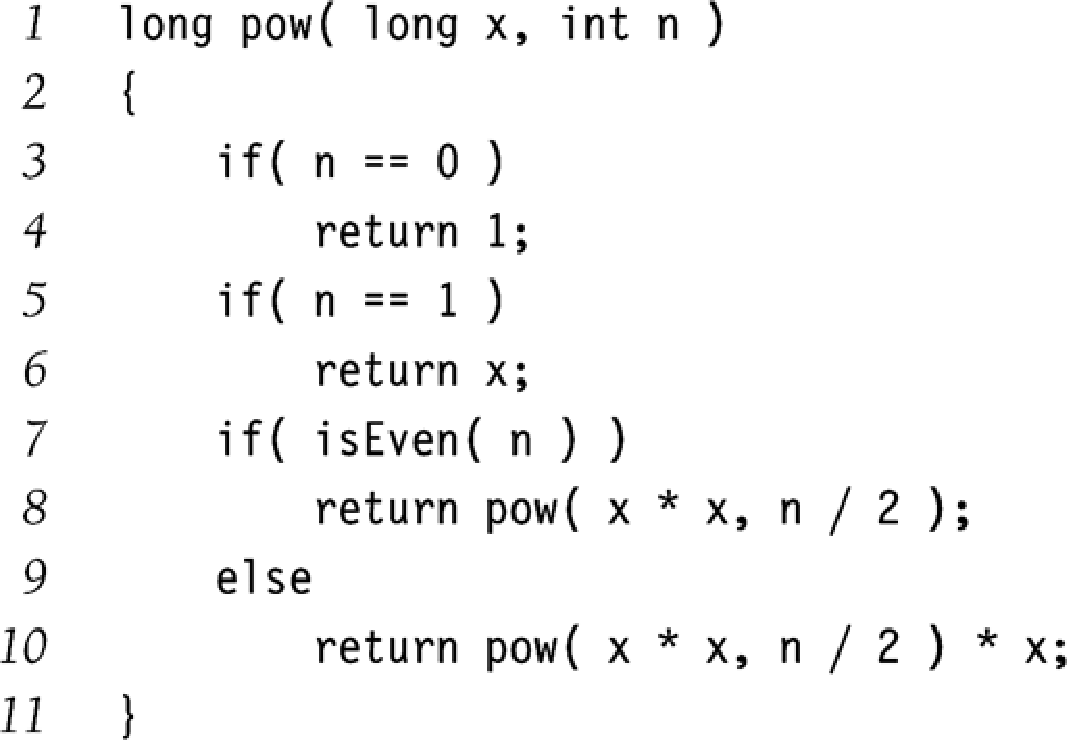
\includegraphics[width=0.6\textwidth]{complexity-figs/exponentiation}
  % \end{figure}
\end{frame}



\begin{frame}
  \frametitle{Complexity of Exponentiation}
  \begin{itemize}
  \item The analysis is simplified by assuming $n=2^k$ (other cases
    are similar, albeit more complicated)
  \item Assume: $n/2$, $half*half$ and the if stmt each costs 1.
  \item for a total of 4 (including the test for x==0) when $n$ is even and 5 when it is odd.
\item Let $T(n)$ be the computational cost for $x^n$ then
  \begin{align*}
 T(n) &=T(n/2)+4\\
      &=T(n/4)+8\\
      &=T(n/2^i)+4i\\
      &=\ldots\\
      &=T(1)+4k\\
      &=\Theta(k)=\Theta(\log n)
  \end{align*}

  \end{itemize}
\end{frame}
\begin{frame}
  \frametitle{Exponentiation}
  \begin{itemize}
  \item In the general case we perform one extra computation every time the exponent is odd.
  \item Let $\beta(n)$ be the number of times such computation is performed.
  \item It is easy to check that $\beta(n)=$ is one less than the number of 1's in the binary representation of $n$
  \item For example if $n=21$ then $21\rightarrow 10\rightarrow 5\rightarrow 2\rightarrow 1$ which means the intermediate value is odd twice.
  \item Compare with the binary representation $21=1011$.
  \item Clearly $\beta(n)$ is at most equal to the number of bits in the binary representation of $n$ which is $\lfloor\log n\rfloor$
\item So even in the general case the complexity is $\Theta(\log n)$.
  \end{itemize}
\end{frame}
\begin{frame}
  \frametitle{General case}
  \begin{itemize}
  \item In general the problem has the following recursion relation
    \begin{displaymath}
      T(n)=T(\lfloor n/2\rfloor)+4+ (n\mod 2)
    \end{displaymath}
\item We will show that the general form
  \begin{align}
\label{eq:2}
      T(n)=T(\lfloor n/2\rfloor)+M+ (n\mod 2)
  \end{align}
\item Has solution
  \begin{align}
\label{eq:1}
    T(n)=M\lfloor \log n\rfloor+\beta(n)
  \end{align}
\item Where $\beta(n)$ is the number of 1's in the binary
  representation of $n$.
\item Using the fact that $\lfloor\log\lfloor
  n/2\rfloor\rfloor=\lfloor \log n\rfloor -1$ it is easy to check that
  \eqref{eq:1} satisfies \eqref{eq:2}.
  \end{itemize}
\end{frame}
\begin{frame}
  \frametitle{Fibonacci: Take Three}
  \begin{itemize}
  \item The previous method for exponentiation can be used to compute
    Fibonacci (n) in $O(\log n)$.
 \item The key is that 
   \begin{displaymath}
    \left(
    \begin{array}{cc}
     F_{n+1} & F_n\\
     F_n    & F_{n-1}
    \end{array}
   \right)
   =
     \left(
    \begin{array}{cc}
     1 & 1\\
     1 & 0
    \end{array}
    \right)^n
   \end{displaymath}
  \item The above is shown by induction on $n$.
   \item We know how to compute the power in $\log n$.
  \end{itemize}
\end{frame}
\end{document}

%%% Local Variables: 
%%% mode: late
%%% TeX-master: t
%%%
